% Options for packages loaded elsewhere
\PassOptionsToPackage{unicode}{hyperref}
\PassOptionsToPackage{hyphens}{url}
\PassOptionsToPackage{dvipsnames,svgnames*,x11names*}{xcolor}
%
\documentclass[
  english,
  a4paper,
  openany]{book}
\usepackage{amsmath,amssymb}
\usepackage[]{bookman}
\usepackage{ifxetex,ifluatex}
\ifnum 0\ifxetex 1\fi\ifluatex 1\fi=0 % if pdftex
  \usepackage[T1]{fontenc}
  \usepackage[utf8]{inputenc}
  \usepackage{textcomp} % provide euro and other symbols
\else % if luatex or xetex
  \usepackage{unicode-math}
  \defaultfontfeatures{Scale=MatchLowercase}
  \defaultfontfeatures[\rmfamily]{Ligatures=TeX,Scale=1}
\fi
% Use upquote if available, for straight quotes in verbatim environments
\IfFileExists{upquote.sty}{\usepackage{upquote}}{}
\IfFileExists{microtype.sty}{% use microtype if available
  \usepackage[]{microtype}
  \UseMicrotypeSet[protrusion]{basicmath} % disable protrusion for tt fonts
}{}
\makeatletter
\@ifundefined{KOMAClassName}{% if non-KOMA class
  \IfFileExists{parskip.sty}{%
    \usepackage{parskip}
  }{% else
    \setlength{\parindent}{0pt}
    \setlength{\parskip}{6pt plus 2pt minus 1pt}}
}{% if KOMA class
  \KOMAoptions{parskip=half}}
\makeatother
\usepackage{xcolor}
\IfFileExists{xurl.sty}{\usepackage{xurl}}{} % add URL line breaks if available
\IfFileExists{bookmark.sty}{\usepackage{bookmark}}{\usepackage{hyperref}}
\hypersetup{
  pdftitle={Bookdown template},
  pdfauthor={Diego Chiquero Mena},
  pdflang={en},
  pdfkeywords={Bookdown, pdf, epub, manual, book},
  colorlinks=true,
  linkcolor=blue,
  filecolor=Maroon,
  citecolor=Blue,
  urlcolor=Blue,
  pdfcreator={LaTeX via pandoc}}
\urlstyle{same} % disable monospaced font for URLs
\usepackage[top=1in,bottom=1in,right=1in,left=1in]{geometry}
\usepackage{longtable,booktabs,array}
\usepackage{calc} % for calculating minipage widths
% Correct order of tables after \paragraph or \subparagraph
\usepackage{etoolbox}
\makeatletter
\patchcmd\longtable{\par}{\if@noskipsec\mbox{}\fi\par}{}{}
\makeatother
% Allow footnotes in longtable head/foot
\IfFileExists{footnotehyper.sty}{\usepackage{footnotehyper}}{\usepackage{footnote}}
\makesavenoteenv{longtable}
\usepackage{graphicx}
\makeatletter
\def\maxwidth{\ifdim\Gin@nat@width>\linewidth\linewidth\else\Gin@nat@width\fi}
\def\maxheight{\ifdim\Gin@nat@height>\textheight\textheight\else\Gin@nat@height\fi}
\makeatother
% Scale images if necessary, so that they will not overflow the page
% margins by default, and it is still possible to overwrite the defaults
% using explicit options in \includegraphics[width, height, ...]{}
\setkeys{Gin}{width=\maxwidth,height=\maxheight,keepaspectratio}
% Set default figure placement to htbp
\makeatletter
\def\fps@figure{htbp}
\makeatother
\setlength{\emergencystretch}{3em} % prevent overfull lines
\providecommand{\tightlist}{%
  \setlength{\itemsep}{0pt}\setlength{\parskip}{0pt}}
\setcounter{secnumdepth}{5}
\usepackage{graphicx}
\usepackage{fancyhdr}
\pagestyle{plain}
\renewcommand{\headrulewidth}{0.2pt}
\usepackage{floatpag}
\floatpagestyle{empty}
\ifxetex
  % Load polyglossia as late as possible: uses bidi with RTL langages (e.g. Hebrew, Arabic)
  \usepackage{polyglossia}
  \setmainlanguage[]{english}
\else
  \usepackage[main=english]{babel}
% get rid of language-specific shorthands (see #6817):
\let\LanguageShortHands\languageshorthands
\def\languageshorthands#1{}
\fi
\ifluatex
  \usepackage{selnolig}  % disable illegal ligatures
\fi
\usepackage[]{natbib}
\bibliographystyle{apalike}

\title{Bookdown template}
\author{Diego Chiquero Mena}
\date{28 enero 2021}

\begin{document}
\maketitle

\thispagestyle{empty}
\begin{center}
\noindent\makebox[\textwidth]{
\includegraphics[width=\paperwidth]{images/cover.png}}
\end{center}
\fontsize{14}{16}
\selectfont





{
\hypersetup{linkcolor=}
\setcounter{tocdepth}{3}
\tableofcontents
}
\hypertarget{prologue}{%
\chapter*{Prologue}\label{prologue}}
\addcontentsline{toc}{chapter}{Prologue}

Bookdown template to write your book and read online, download PDF or ePub (ebook) format from top menu options of online version.

PDF and ePub format output already setup. Ready to write your words, ideas, thoughts or whatever thing you want to tell us?.

This book have been writing with \href{http://rmarkdown.rstudio.com}{R-Markdown} and\href{https://bookdown.org/}{\texttt{bookdown}} package and its guide you will find on \citep{R-bookdown}.

This link goes to other books made with \href{https://bookdown.org/home/archive/}{Bookdown}.

IDE (integrated development environment) recommended \href{https://rstudio.com/products/rstudio/download/}{RStudio}, but choose yours.

Image cover \citep{photopea}

This work is under license \href{https://creativecommons.org/licenses/by-nc-sa/4.0/deed.es}{licencia Creative Commons Atribución-NoComercial-CompartirIgual 4.0 Internacional}. But choose your \href{https://creativecommons.org/}{License Creative Commons}.

\begin{flushleft}
\includegraphics{images/by-nc-sa-88x31} \end{flushleft}

\hypertarget{author}{%
\chapter*{About the author}\label{author}}
\addcontentsline{toc}{chapter}{About the author}

\begin{flushleft}
\includegraphics[width=0.25\linewidth]{images/photo-profile} \end{flushleft}

Hello, my name is Elise.

Lorem ipsum dolor sit amet, consectetur adipiscing elit, sed do eiusmod tempor incididunt ut labore et dolore magna aliqua. Ut enim ad minim veniam, quis nostrud exercitation ullamco laboris nisi ut aliquip ex ea commodo consequat.

\begin{quote}
Write your quote here
\end{quote}

My contact \href{mailto:fur.elise@mail.es}{\nolinkurl{fur.elise@mail.es}}

More about me \href{https://about.me/}{Elisa}

\hypertarget{intro}{%
\chapter{Introduction}\label{intro}}

Lorem Ipsum is simply dummy text of the printing and typesetting industry. Lorem Ipsum has been the industry's standard dummy text ever since the 1500s, when an unknown printer took a galley of type and scrambled it to make a type specimen book. It has survived not only five centuries, but also the leap into electronic typesetting, remaining essentially unchanged. It was popularised in the 1960s with the release of Letraset sheets containing Lorem Ipsum passages, and more recently with desktop publishing software like Aldus PageMaker including versions of Lorem Ipsum.

\hypertarget{label-chapter}{%
\chapter{Label chapter}\label{label-chapter}}

You can label chapter and section titles using \texttt{\{\#label\}} after them, e.g., we can reference Chapter \ref{intro}. If you do not manually label them, there will be automatic labels anyway, e.g., Chapter \ref{levels}.

\hypertarget{image}{%
\chapter{Image}\label{image}}

Here you are seeing below image. Beautiful, isn't it?

Add or remove its title. It's up to you.

\begin{figure}

{\centering 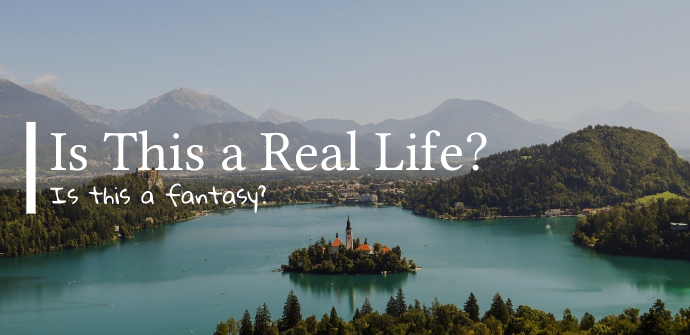
\includegraphics[width=1\linewidth]{images/photo-example} 

}

\caption{Photo example template.}\label{fig:rmarkdown}
\end{figure}

\hypertarget{hyperlink}{%
\chapter{Hyperlink}\label{hyperlink}}

Hyperlink example to go \href{https://www.google.com}{Google} right now.

\hypertarget{footnotes}{%
\chapter{Footnotes}\label{footnotes}}

Show me a simple footnotes\footnote{Here it is your simple footnotes}.

Other way to create a footnotes\footnote{Your footnotes is shown.}.

Footnotes with links\footnote{Other guides \href{https://bookdown.org/yihui/rmarkdown-cookbook/}{R Markdown Cookbook} and \href{https://bookdown.org/yihui/rmarkdown/}{The definitive guide}}

At vero eos et accusamus et iusto odio dignissimos ducimus qui blanditiis praesentium voluptatum deleniti atque corrupti quos dolores et quas molestias excepturi sint occaecati cupiditate non provident, similique sunt in culpa qui officia deserunt mollitia animi, id est laborum et dolorum fuga. Et harum quidem rerum facilis est et expedita distinctio.

Nam libero tempore, cum soluta nobis est eligendi optio cumque nihil impedit quo minus id quod maxime placeat facere possimus, omnis voluptas assumenda est, omnis dolor repellendus. Temporibus autem quibusdam et aut officiis debitis aut rerum necessitatibus saepe eveniet ut et voluptates repudiandae sint et molestiae non recusandae.

Itaque earum rerum hic tenetur a sapiente delectus, ut aut reiciendis voluptatibus maiores alias consequatur aut perferendis doloribus asperiores repellat.

\hypertarget{link-to-bibliography}{%
\chapter{Link to bibliography}\label{link-to-bibliography}}

This is an example of reference or bibliography source \citep{example-ref} that will take you to wikipedia bibliography definition, managed from \emph{manual.bib} file.

Another sample of reference o bibliography source \citep{article} managed from \emph{article.bib} file.

\begin{verbatim}
You can add text to your text as follows.
\end{verbatim}

\hypertarget{levels}{%
\chapter{Deep levels}\label{levels}}

Some \emph{examples} of deep levels.

Sed ut perspiciatis unde omnis iste natus error sit voluptatem accusantium doloremque laudantium, totam rem aperiam, eaque ipsa quae ab illo inventore veritatis et quasi architecto beatae vitae dicta sunt explicabo.

\hypertarget{second-level-a}{%
\section{Second level A}\label{second-level-a}}

Nemo enim ipsam voluptatem quia voluptas sit aspernatur aut odit aut fugit, sed quia consequuntur magni dolores eos qui ratione voluptatem sequi nesciunt.

\hypertarget{third-level}{%
\subsection{Third level}\label{third-level}}

Neque porro quisquam est, qui dolorem ipsum quia dolor sit amet, consectetur, adipisci velit, sed quia non numquam eius modi tempora incidunt ut labore et dolore magnam aliquam quaerat voluptatem.

\hypertarget{fourth-level}{%
\subsubsection{Fourth level}\label{fourth-level}}

Ut enim ad minima veniam, quis nostrum exercitationem ullam corporis suscipit laboriosam, nisi ut aliquid ex ea commodi consequatur? Quis autem vel eum iure reprehenderit qui in ea voluptate velit esse quam nihil molestiae consequatur, vel illum qui dolorem eum fugiat quo voluptas nulla pariatur?.

\hypertarget{second-level-b}{%
\section{Second level B}\label{second-level-b}}

An so on\ldots{}

  \bibliography{book.bib,article.bib,manual.bib}

\end{document}
